\subsection*{EURIO: EUropean Research Information Ontology}
The \gls{eurio} ontology, developed by the Publications Office of the European Union\footnote{\url{https://op.europa.eu/en/}}, is a data model which conceptualizes, formally encodes, and makes available in an open, structured, and machine-readable format data about research projects funded by the EU's framework programmes for research and innovation.
\gls{cordis} is responsible for publishing the results of these projects, while \gls{eurio} provides a semantic model that enhances transparency, reusability, and accessibility.
The \gls{eurio} ontology is built on top of well-known ontologies and vocabularies to ensure interoperability and semantic richness.
These include:
\begin{itemize}
    \item \gls{dc}: used for metadata elements such as titles, descriptions, and identifiers.
    \item \gls{dcat}: an \gls{rdf} vocabulary designed to facilitate interoperability between data catalogs published on the Web.
    \item \gls{dingo}: an ontology expressly designed to provide an extensible interoperable framework for formally conceptualizing and expressing the relevant parts of the research/cultural landscape in relation to funding, such that they can easily be shared between different actors and platforms.
    \item \gls{fabio}: facilitates the description of bibliographic entities and their relationships.
    \item \gls{frapo}: an ontology for describing the administrative information of research projects, e.g., grant applications, funding bodies, project partners, etc.
    \item \gls{foaf}: defines relationships between people and organizations.
    \item \gls{skos}: facilitates controlled vocabularies and classification schemes.
\end{itemize}

The \gls{eurio} Ontology also incorporates reference data, such as countries, funding schemes, types of action, the EuroSciVoc taxonomy, and the NUTS classification, to enhance the semantic representation of research information.
It leverages the \gls{owl} 2 to formally define the semantics of domain-specific terms used to describe \gls{cordis} entities (e.g., projects, organizations, etc.), their attributes (e.g., title, acronym, legal name, etc.), and their interrelations (e.g., the connection between a project and its participating organizations, etc.).

\gls{eurio} is part of the EU's reference data assets, which include ontologies, thesauri, taxonomies, and authority tables.
These structured data assets improve the visibility, reusability, and accessibility of research information.
The \gls{eurio} ontology defines multiple classes representing different concepts such as projects, organizations, funding schemes, grants, publications, and roles, along with associated data properties and object properties that define their relationships.
Each class has a set of data properties that describe its attributes, and a set of object properties that define its connections to other classes.
Each class, data property, and object property has several annotations but in general the main annotations for those are rdfs:label, which provides a human-readable label for the entity, rdfs:comment, which provides a human-readable description of the entity, and rdfs:isDefinedBy, which provides a link to the ontology where the entity is defined.
For example, the title, description, start date, end date, and funding amount are data properties of the \textbf{Project} class.

\begin{figure}[htbp]
    \centering
 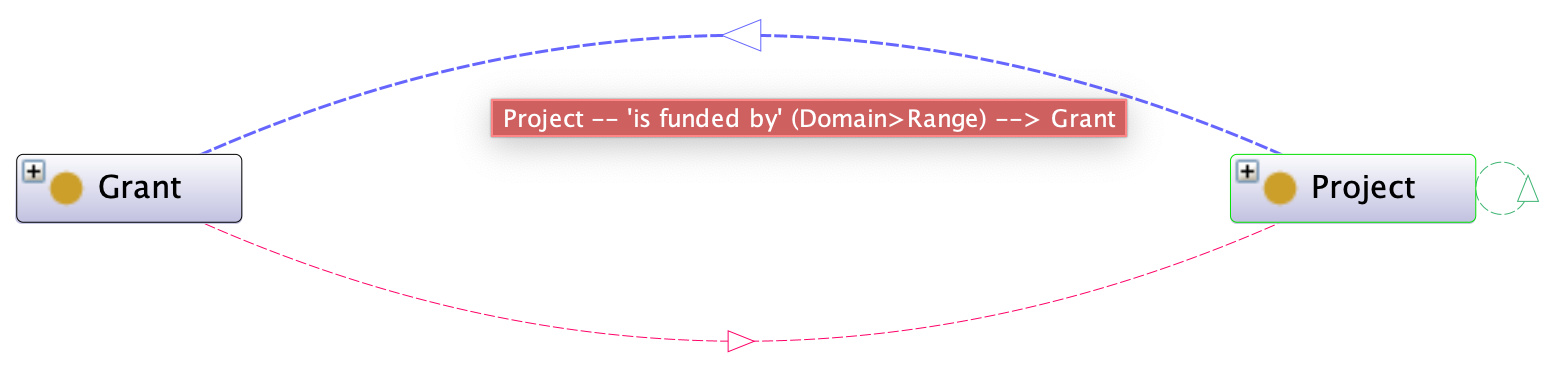
\includegraphics[width=\textwidth]{figures/data-analysis/is-funded-by.png}
     \rule{35em}{0.5pt}
    \caption{The ``is funded by'' relationship between a project and its grant}
 \label{fig:is-funded-by}
\end{figure}

The ontology also defines relationships between classes, such as \textbf{is funded by}, the association between a project and its grant (Fig.~\ref{fig:is-funded-by}).
Another example or relationship is \textbf{is employed by}, which links a person, in particular a \textbf{Person Role} to an \text{Organisation}.
The ontology also provides object property descrptions, for example the \textbf{has involved party} relationship, which links a \textbf{Project} to a \textbf{Role}, is inverse of \textbf{is involved in}, which links a \textbf{Role} to a \textbf{Project} (Fig.~\ref{fig:is-involved-in-has-involved-party}).

\begin{figure}[htbp]
    \centering
 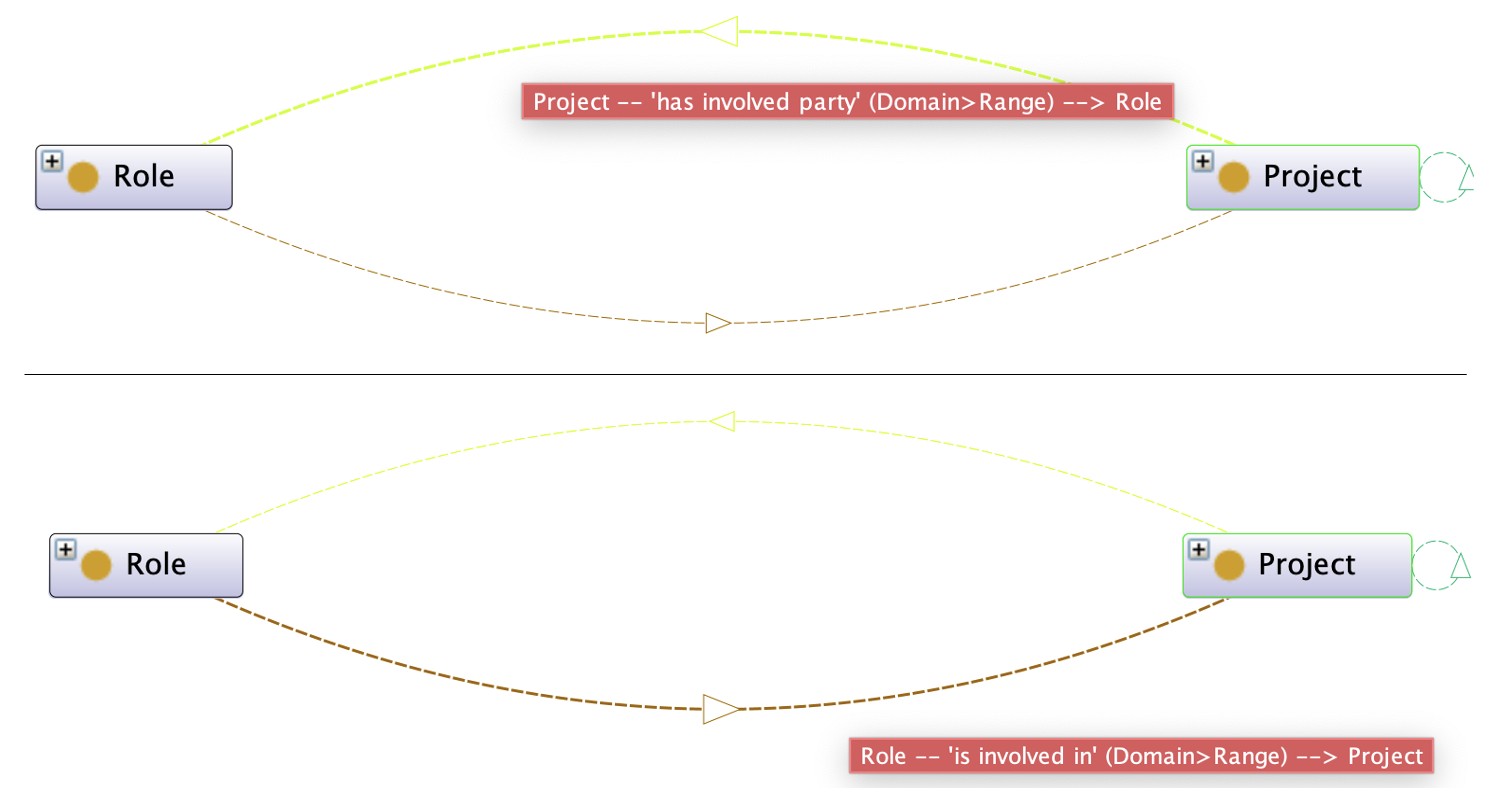
\includegraphics[width=\textwidth]{figures/data-analysis/has-involved-party-is-involved-in.png}
     \rule{35em}{0.5pt}
    \caption{The ``has involved party'' and ``is involved in'' relationships}
 \label{fig:is-involved-in-has-involved-party}
\end{figure}

This object property descriptions can be very useful for querying the \gls{kg} to extract relevant information in a structured manner.
Moreover, the ontology defines a hierarchy of classes.
For example, the \textbf{Organisation} class is a superclass of several subclasses such as \textbf{For Profit Organisation}, \textbf{Funding Agency}, \textbf{Higher Or Secondary Education}, \textbf{Research Organisation}, and \textbf{SME} (Small and Medium Enterprise) (Fig.~\ref{fig:organisation-class-hierarchy}).

\begin{figure}[htbp]
    \centering
 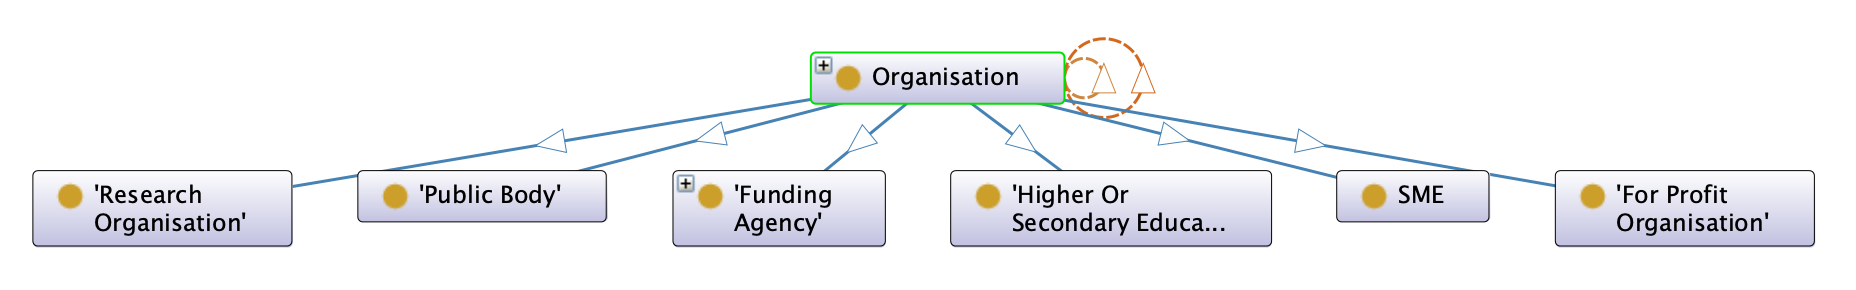
\includegraphics[width=\textwidth]{figures/data-analysis/organisation-class-hierarchy.png}
     \rule{35em}{0.5pt}
    \caption{The ``Organisation'' class hierarchy}
 \label{fig:organisation-class-hierarchy}
\end{figure}

An overview of the \gls{eurio} ontology is shown in the UML diagram in Fig.~\ref{fig:eurio-ontology}.

\begin{figure}[htbp]
    \centering
 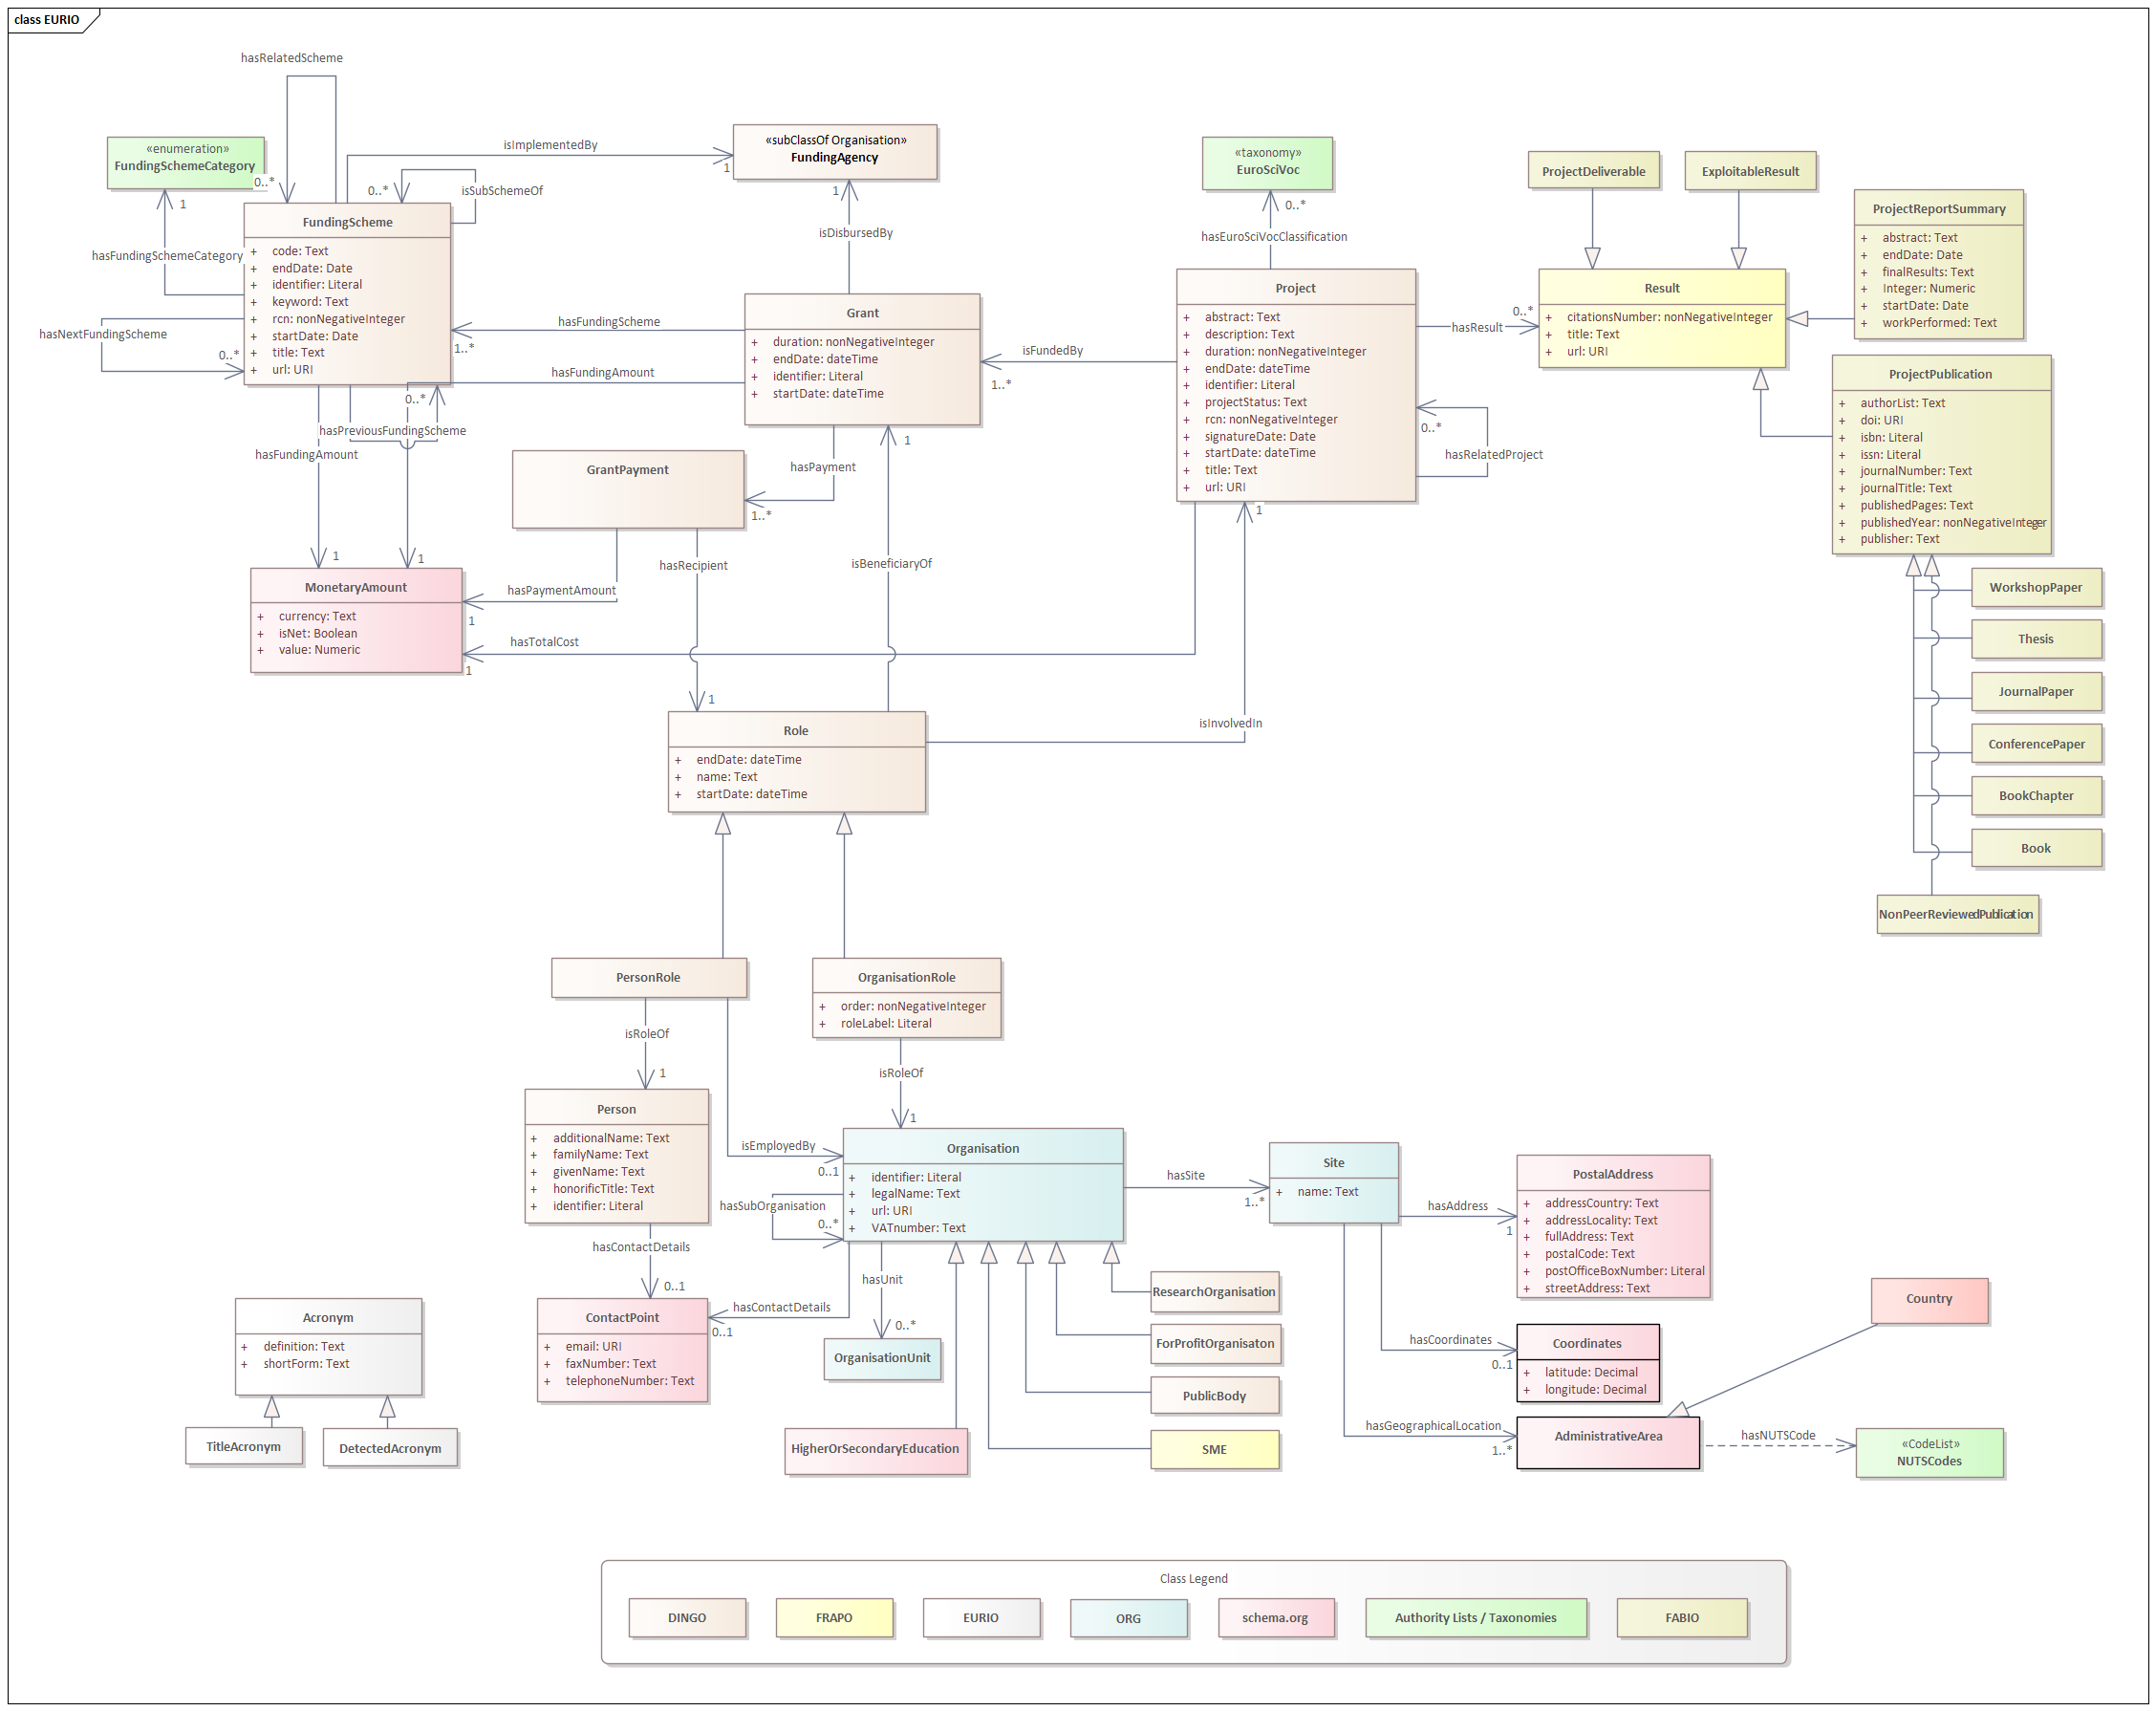
\includegraphics[width=\textwidth]{figures/data-analysis/EURIO_V2.4.png}
     \rule{35em}{0.5pt}
    \caption{A graphical representation of the \gls{eurio} ontology (from \url{https://op.europa.eu/en/web/eu-vocabularies/eurio})}
 \label{fig:eurio-ontology}
\end{figure}

\subsection*{Data Availability and Formats}

The \gls{eurio} dataset is available in multiple formats to ensure accessibility and ease of integration into different research workflows.
Supported formats include \gls{rdf}, \gls{ttl}, \gls{nq}, \gls{jsonld}, and \gls{nt}.
The \gls{eurio} \gls{kg} used in this thesis is the latest version updated by the European Union on 08.11.2023, ensuring that the data remains relevant and accurate up to this date.

\section{\gls{eurio} Knowledge Graph Exploration}

TODO: inserire tutti gli aspetti trovati analizzando eurio, inclusi problemi, dati mancanti, dati ridondanti etc.

TODO: inserire screen di vari sottografi all'interno di eurio.


\begin{figure}[htbp]
    \centering
 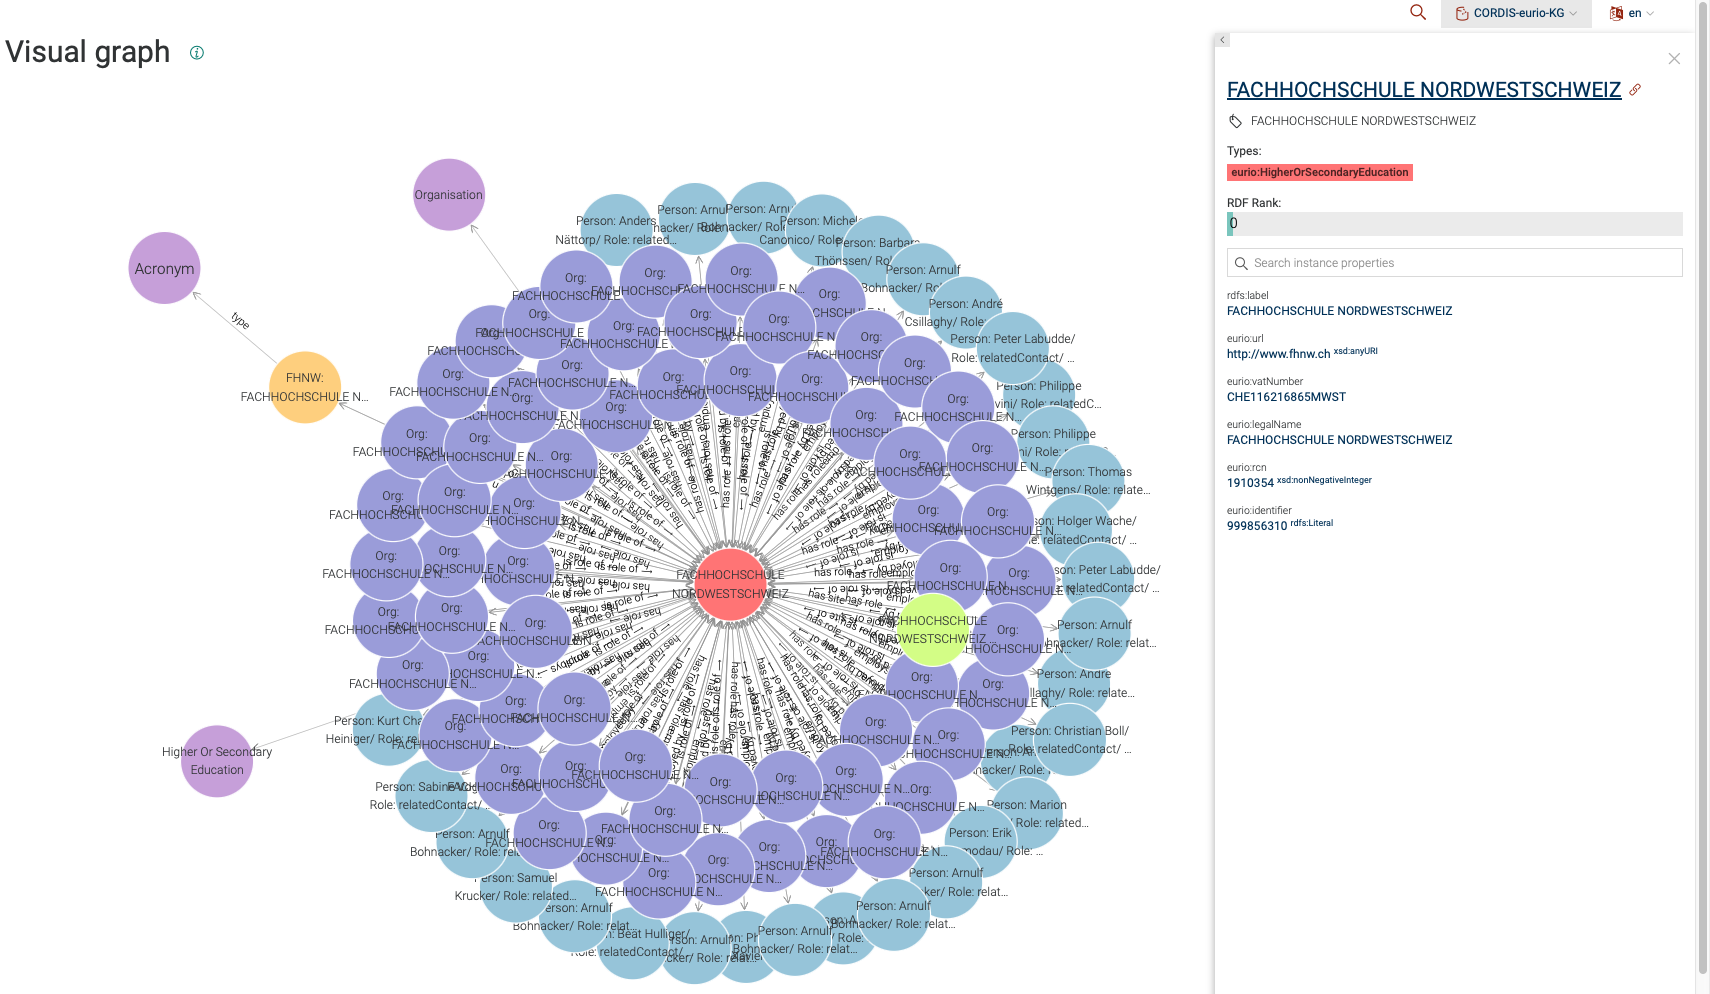
\includegraphics[width=\textwidth]{figures/data-analysis/graphdb-fhnw.png}
     \rule{35em}{0.5pt}
    \caption{FACHHOCHSCHULE NORDWESTSCHWEIZ (FHNW) subgraph in the \gls{eurio} \gls{kg}}
 \label{fig:fhnw-graphdb}
\end{figure}

\begin{figure}[htbp]
    \centering
 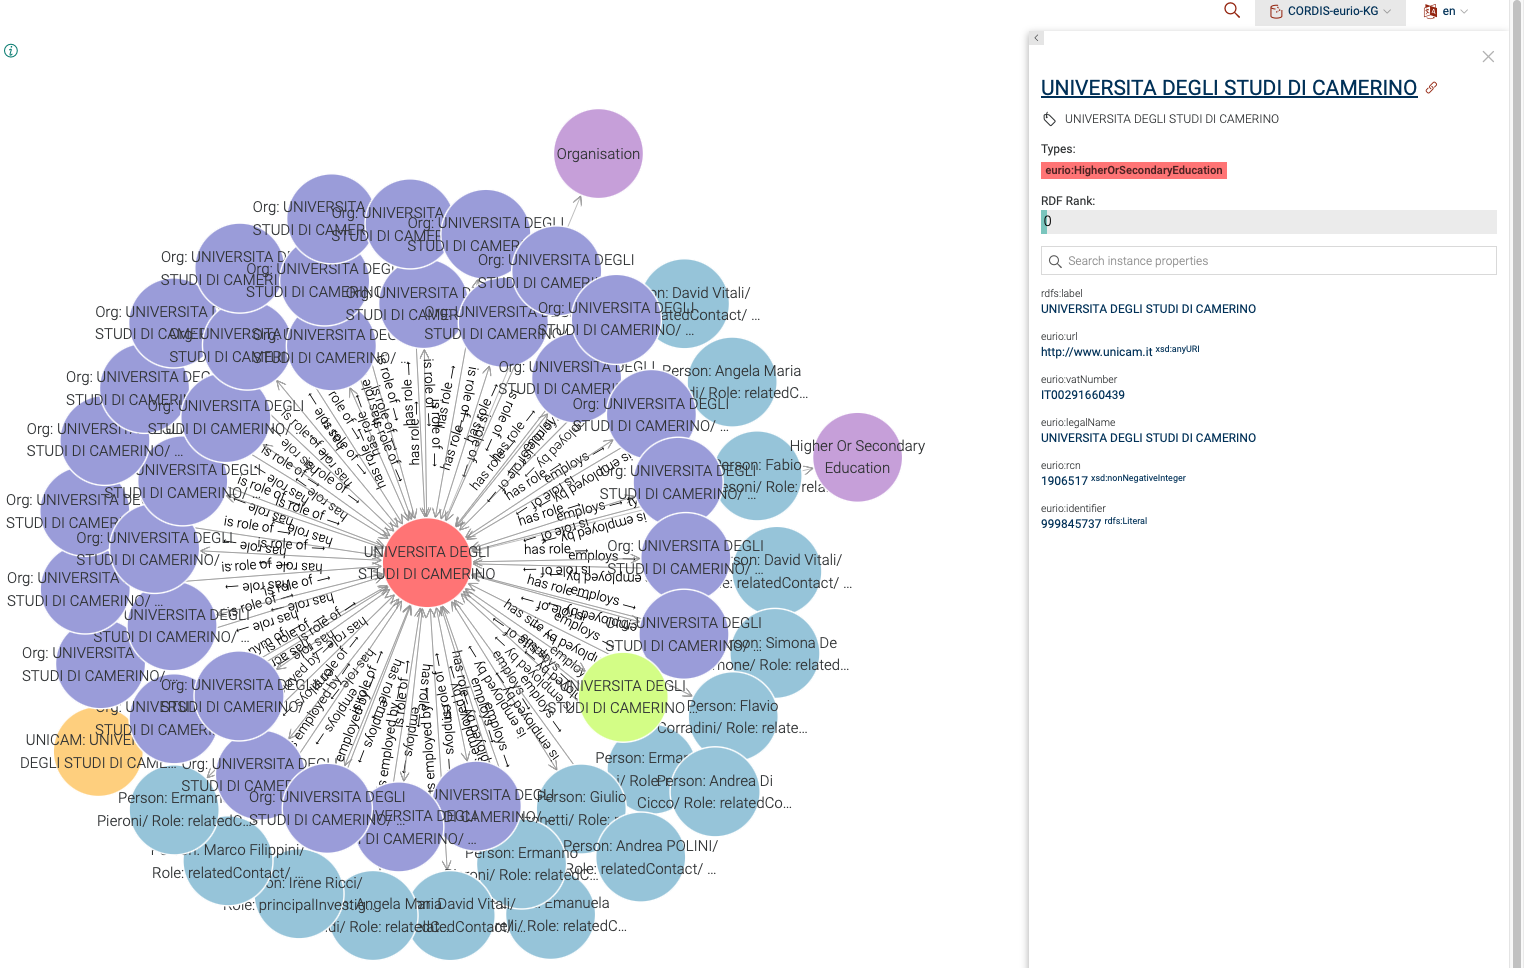
\includegraphics[width=\textwidth]{figures/data-analysis/graphdb-unicam.png}
     \rule{35em}{0.5pt}
    \caption{University of Camerino (UNICAM) subgraph in the \gls{eurio} \gls{kg}}
 \label{fig:unicam-graphdb}
\end{figure}